% Created 2022-04-04 Mon 10:24
% Intended LaTeX compiler: pdflatex
\documentclass[11pt]{article}
\usepackage[utf8]{inputenc}
\usepackage[T1]{fontenc}
\usepackage{graphicx}
\usepackage{longtable}
\usepackage{wrapfig}
\usepackage{rotating}
\usepackage[normalem]{ulem}
\usepackage{amsmath}
\usepackage{amssymb}
\usepackage{capt-of}
\usepackage{hyperref}
\usepackage{minted}
\author{Rémi Louf}
\date{\today}
\title{The typical set}
\hypersetup{
 pdfauthor={Rémi Louf},
 pdftitle={The typical set},
 pdfkeywords={},
 pdfsubject={},
 pdfcreator={Emacs 27.2 (Org mode 9.6)}, 
 pdflang={English}}
\begin{document}

\maketitle
\tableofcontents

👋 I am Rémi (\href{mailto:remi@thetypicalset.com}{email}, \href{https://twitter.com/remilouf}{twitter})

You've just stepped on \textbf{the typical set}, a subset of my personal notes, my blog, and some longform write ups. Feel
free to explore. You can start with what I am doing now and what I am working
on.

I am a glorified statistician (some say \href{https://hbr.org/2012/10/data-scientist-the-sexiest-job-of-the-21st-century}{data scientists}) and software developer. I am currently a very busy freelance. I am particularly interested in bayesian statistics \& generative modeling, mcmc sampling and symbolic computing, which translate into my professional life and the open source projects I contribute to:

\begin{itemize}
\item \href{https://github.com/blackjax-devs/blackjax}{Blackjax} is a sampling (mostly MCMC) library that is built with JAX for ease of use, speed and modularity.
\item \href{https://github.com/aesara-devs/aemcmc}{Aemcmc} is a sampling library built with Aesara which builds samplers from model graphs. \href{https://github.com/aesara-devs/aehmc}{Aehmc}
implements symbolic HMC and NUTS samplers, but will likely merge into Aemcmc.
\item \href{https://github.com/rlouf/mcx}{MCX} is an experimental PPL, deprecated in favor of Blackjax and Aesara/Aeppl. \href{blog/introducing-mcx.org}{Read the blog post}.
\end{itemize}


Unlike a traditional blog, most of the notes you will find here are \textbf{constant
work in progress}. They are mostly written for myself. Many of them are stubs,
ideas waiting to be explored. They coalesce in \href{blog/index.org}{blog posts} (which are often
\emph{timely}) or longer \href{file:///home/remi/projects/blog/.dir-locals.el}{projects} which aim at being evergreen bur are written for others.

With this experiment I am also trying to figure out how to write useful notes, and how to
efficiently navigate between them.

These notes are generated with \href{https://www.orgroam.com/}{Org-roam} and are automatically published with \href{https://www.orgmode.org/fr/}{Org Mode}.

\section{What I'm currently reading}
\label{sec:org3f28031}

\begin{center}

\includegraphics[width=.9\linewidth]{img/books/jackson-de-gaulle.jpg}
\end{center}

\begin{center}
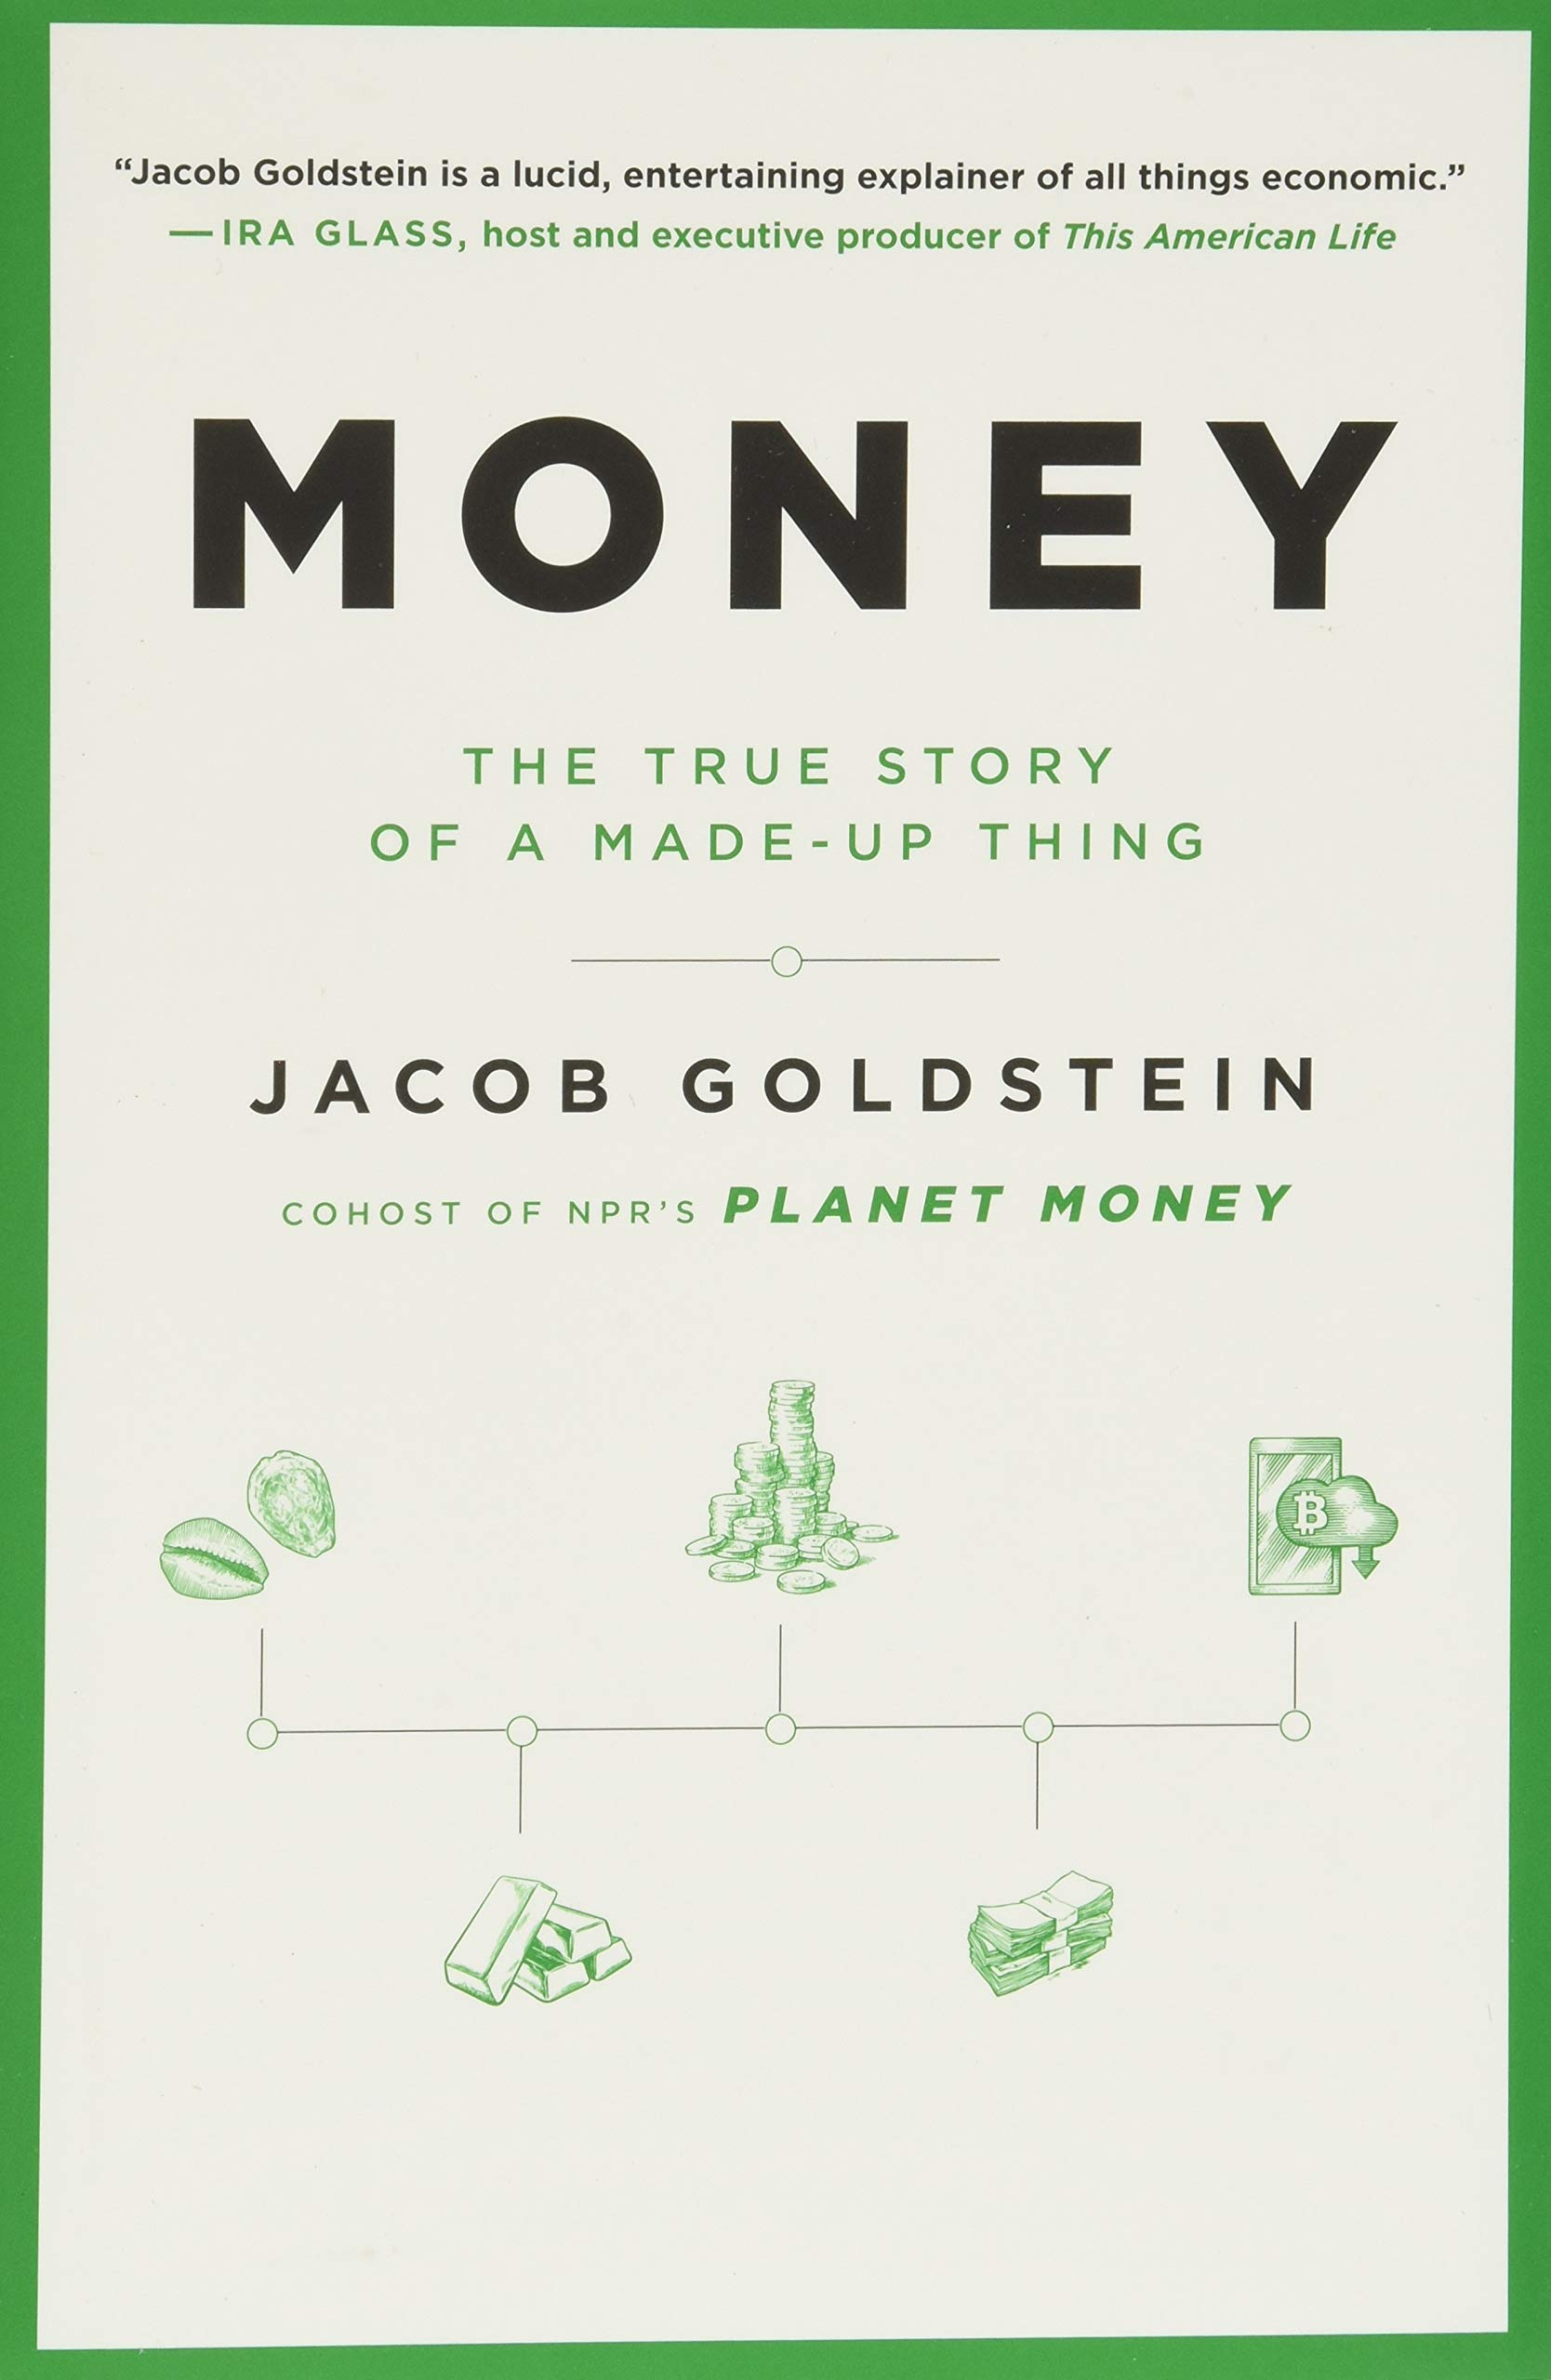
\includegraphics[width=.9\linewidth]{img/books/goldstein-money.jpg}
\end{center}

\begin{center}
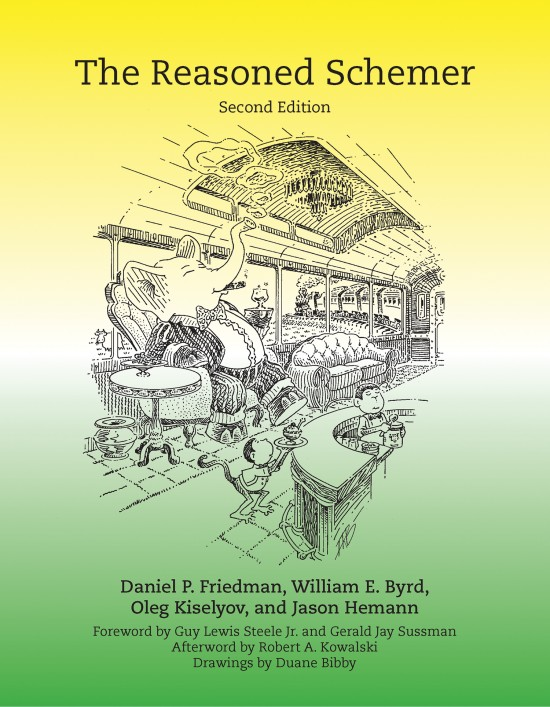
\includegraphics[width=.9\linewidth]{img/books/friedman-reasoned-schemer.jpg}
\end{center}
\end{document}
